\chapter{Projektbeskrivelse}
\section{Projektgennemførelse}
 
Dette projekt er gennemført vha. forskellige udviklingsprocessor, hvilket er med til at sikre kvalitet, og at deadlines overholdes. En af disse modeller er ASE-modellen \cite{ISE}. Denne model er en udviklingsmodel, der er udarbejdet af Aarhus Ingeniørhøjskole. Modellen er en semi-iterativ udviklingsproces drevet ud fra projektets Use Cases. Modellen er benyttet på den måde, at gruppemedlemmerne fastlægger en projektformulering, kravspecifikation og systemarkitektur, for derefter at designe og implementere de enkelte hardware og software dele. Gennem en integrations test ses det om hardware og software delene fungere.  
Dette ender med en gennemført accepttest, således at det testes om systemet lever op til kravene og der opnås en enighed mellem projektmedlemmer og forsker.
\begin{figure}[H]
	\centering
	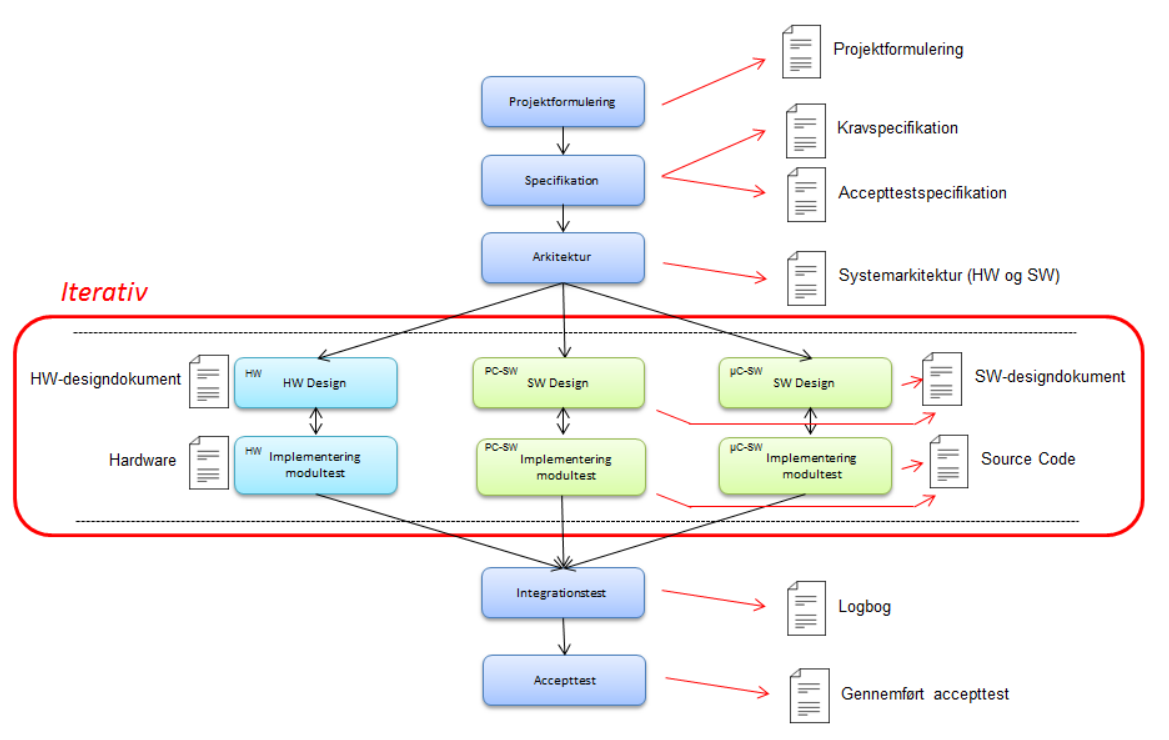
\includegraphics[width=0.8\textwidth]{Figurer/AseModellen}
	\caption{ASE-modellen}
	\label{fig:ASE_model}
\end{figure}
For at forstå ASE-modellen \cite{ISE} er det vigtigt at gennemgå Use Cases; et værktøj, som skal beskrive interaktioner mellem diverse aktører og selve systemet. Sammen med de ikke-funktionelle krav opnås et overblik over hvilke funktionalitetskrav, der stilles til systemet. På baggrund af kravspecifikationen kan accepttesten efterfølgende udarbejdes. I dette projekt er hardware- og software design implementering på lige fod, da projektet består af begge ting ligeligt.\\
\newline
V-modellen \cite{ISE} er en faseopdelt udviklingsmodel, der også er værd at nævne i dette projekt. Den beskriver udviklingsfaserne og testfaserne sideløbende i forhold til projektet, og den er derfor benyttet til dette projekt sideløbende med ASE-modellen. Modellen fungerer således, at specifikationen af test foregår parallelt med udviklingen af selve systemet.

\begin{figure}[H]
	\centering
	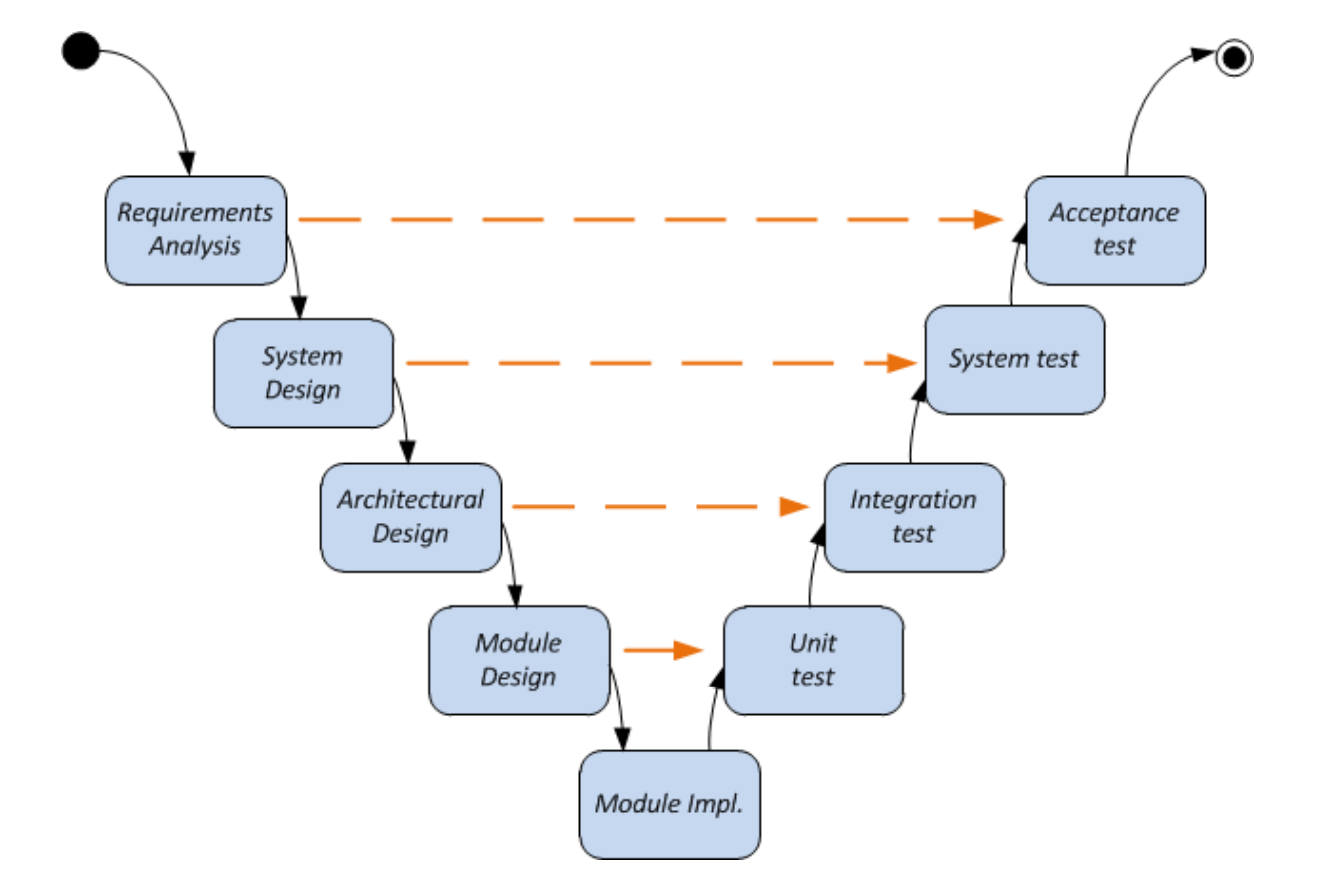
\includegraphics[width=0.6\textwidth]{Figurer/VModellen}
	\caption{V-model}
	\label{fig:V_Modellen}
\end{figure}

Den er blevet benyttet til hardware og software udviklingen. Hardware og software skulle begge teste deres funktioner inden nye faser blev igangsat, for at verificere om disse funktioner virkede korrekt gennem forløbet. Fordelen ved at teste på forskellige niveauer er, at det skal sikre de udviklede delsystemer, således at de virker som planlagt. Det er vigtigt, at hver fase er udført, før den næste fase påbegyndes. 
\newline

Vandfaldsmodellen \cite{ISE} er også blevet benyttet under dette projekt. Softwareudviklingen bærer præg af vandfaldsmodellen, da udviklingen er opdelt i faser, hvor hver fase er blevet gennemført, før den næste er påbegyndt. Dette er i relation til V-modellen, som blev beskrevet før og den er, som vist på figur XX, konstant strømmende nedad. 

\begin{figure}[H]
	\centering
	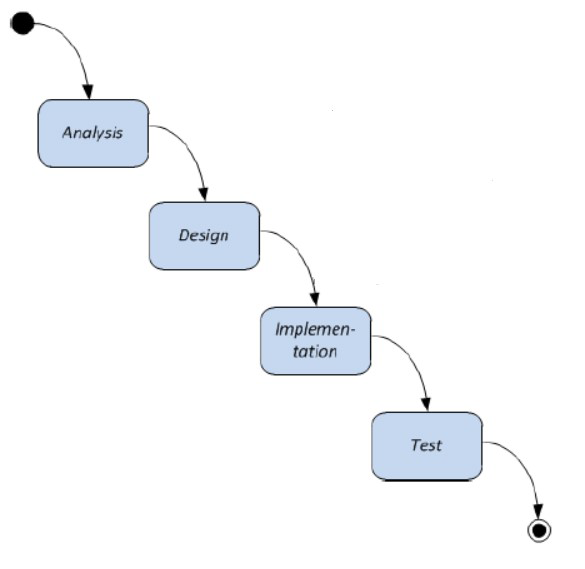
\includegraphics[width=0.4\textwidth]{Figurer/VandfaldsModellen}
	\caption{Vandfalds modellen}
	\label{fig:vandfalds_model}
\end{figure}


\section{Projektstyring}
Projektet er udarbejdet over et helt semester, hvor undervisningen og forelæsningerne delvist har udgjort grundlaget for teorien benyttet i dette projekt. Der blev i starten udarbejdet en tidsplan, som dog var mulig at ændre undervejs, men med faste deadlines, der skulle overholdes. Hovedpunkterne kan ses i denne tidsplan, som er vedlagt i bilag XX. \\
Projektgruppen har bestået af 6 gruppemedlemmer, som er blevet delt i 2 fokusområder, hardware og software.Fordelingen blev udarbejdet efter den enkeltes ønske. Gruppen har derfor været afhængig af at der var god kommunikation mellem de to undergrupper, derfor har hver arbejdsgang været i samarbejde. Da gruppen har været opdelt, har der været projektmøde hver uge, hvor gruppen har opdateret hinanden og vejleder. \\
Under projektet har alle medlemmer været med til, at sikre en administrativ kæde af deadlines til individuelle opgaver, samt dagsordener til hvert møde. Disse deadlines har sikret at opgaverne er blevet opfyldt op til møderne, for at hindre langsomme arbejdsprocesser. Da der har været overlap mellem de forskellige opgaver er arbejdet foregået flydende for at sikre, at der blev testet. 

\section{Metoder}
Til at kunne overskue arkitektur og designet af projektet, er flere forskellige arbejdsmetoder benyttet for at skabe det bedst mulige resultat. 
For at finde, hvad blodtryksmåleren skal gøre, er der blevet udarbejdet Use Cases. Disse beskriver systemet funktionalitet. Use Cases viser, hvad brugeren skal opleve fra systemet, men ikke, hvordan det sker. I Use Case diagrammet bliver det også vist, hvilke aktører der findes og hvordan de interagerer med systemet.   \\
I projektet bruges accepttest til at teste blodtryksmåleren. Dette gøres ud fra kravspecifikationerne, hvor det er angivet, hvilke krav der er til systemet. \\Accepttesten er en test, hvor der beskrives, hvad der skal ske og, hvad brugeren skal gøre. Testen er for at undersøge om produktet opfylder de krav, som der er blevet sat for det. Accepttesten giver et godt overblik for udvikleren og for kunden, der nemt og hurtigt kan se om produktet virker som det skal. \\
\newline
Til  beskrivelse af design af software og hardware er diagrammer og skemaer blevet udarbejdet i SysML og UML. SysML er et grafisk modelleringssprog, som kan bruges til at overskueliggøre systemer. \\
Til software er der blandt andet lavet en applikationsmodel i SysML, som består af et domæne-, klasse- og sekvensdiagram. \\
Domænemodellen viser sammenhængen mellem blokkene i systemet. Blokkene findes i Use Casene og derved bliver disse to ting koblet sammen. \\
Klassedigrammet viser, hvilke metoder blokkene har og hvordan de kommunikerer med hinanden. Her findes domæne-, kontrol- og grænsefladeklasser. Kontrolklasserne beskriver, hvordan data behandles mellem domæne- og grænsefladeklasser. Domæneklasser indeholder funktionalitet fra den pågældende softwareblok. Grænsefladeklasserne viser, hvordan, systemet interagerer med omverdenen. Diagrammet gør det nemmere at fremme en lav kobling og høj samhørighed i softwaren.\\
Sekvensdiagrammet fortæller, hvad der sker i selve koden. Igen går det ud fra Use Casene, hvor vægten nu er på softwaredelen. Derved beskrives det, hvordan metoder bliver kaldt og hvordan de forskellige klasser interagerer. Hver Use Case skal her gennemgås i software, så der skabes et overblik over vejen gennem koden.\\
\newline 
For at skabe et overblik og indsigt i koden, er der i UML udarbejdet et aktivitetsdiagram og et klassediagram. Aktivitetsdiagrammet går i dybden med en specifik metode. Det er kun blevet gjort for relevante metoder. Her tydeliggøres det, hvordan hver metode fungere og, hvad den indeholder.  Klassediagrammet fortæller hvilke metoder, en klasse indeholder og hvordan klasserne hænger sammen.\\
\newline  
Til hardwaren er der blevet brugt Block Definition Diagram(BDD), som viser hvilke blokke et system indeholder og hvilke porte de har. BDD er lavet til at give et overblik over systemet. Ud fra BDD’et er et Internal Block Diagram(IDB) blevet lavet. Her vises, hvilke signaler som findes i systemet og hvordan de sendes rundt. Her vises portene igen og der skal være overensstemmelse  mellem BDD og IBD.    
\newline 
Til udarbejdelsen af kredsløb blev Analog Discovery brugt til at simulerer signalet, som i sidste ende skal komme fra transduceren. Først blev kredsløbet opbygget på et fumlebræt, hvor det blev testet for at afprøve om det lever op til kravene. Når det opfylder kravene, flyttes det over på et VEVO Board. VEVO Boardet bliver igen testet før aflevering. 

\section{Systemarkitektur}

\begin{figure}[H]
	\centering
	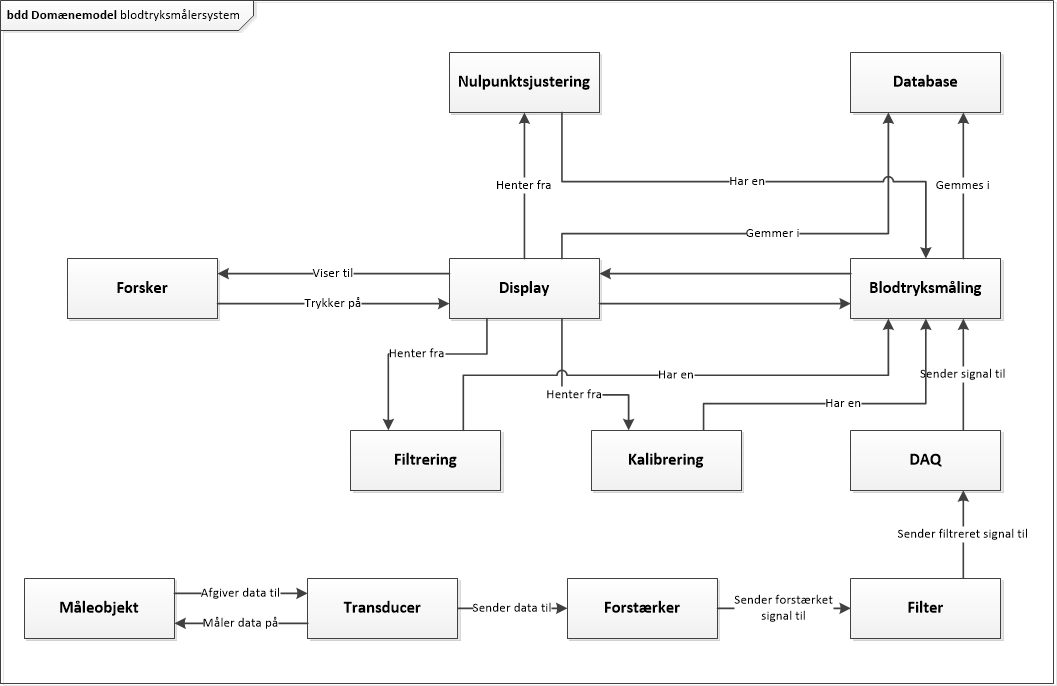
\includegraphics[width=1.0\textwidth]{Figurer/DomaneModel}
	\caption{Domæne Model}
	\label{fig:Domaene Model}
\end{figure}

\subsection{Hardware}
I hardware delen skal der ligge en forstærkning og et lavpasfilter. Det differentieret signal fra transduceren skal forstærkes og filtrers før det kan sendes ind i DAQ'en. Se figur 
\subsection{Software}

\section{Problemidentifikation (design)}
\subsection{Hardware}
\subsubsection{Forstærkning}
Transduceren måler en trykændring som den omsætter til en spænding. Dette er udtrykt ved et differentieret signal, som sendes ind i forstærker-blokken. \\
Signalet fra transduceren er en lav spænding, som skal forstærkes op, for at passe med DAQ'ens input. Denne forstærkning udregnes ud fra det maksimale output fra transduceren og det maksimale input til DAQ'en. Se beregningerne under Implementering.  
\newline
Under simulering bruges Analog Discovery som en funktionsgenerator, der simulere det differentieret signal.  

\subsubsection{Lavpas}
I projektet skal der laves et 2. ordens lavpasfilter. Filteret skal laves for at sikre, at der ikke opstår aliasering.\\
Aliasering \cite{DSB} er, hvor signalet bliver gentaget. Når man har signalet i det digitale domæne, bliver spektret for signalet en periodisk funktion. Det vil sige, at den gentager sig selv, efter et bestemt stykke tid. \\
Det skal sikres, at der ikke kommer overlap mellem signalet og et alias. Da det ellers kunne give anledning til misforståelser. Derfor laves et lavpasfilter, som sikre at der ikke ligger noget signal ved den halve samplingsfrekvens.    
\newline  
Lavpasfilteret skal være et Sallen-Key Butterworth-filter med en knækfrekvens på 50 Hz og en samplingsfrekvens på 1kHz. Ud fra oplysninger givet til projektet, vides det at filteret skal dæmpe signalet med 20 dB, under antagelse af at den forekommende støj er mindre end signalet, også når det  forekommer over knækfrekvensen.\\
Ved en typisk blodtryksmåling forekommer der ikke signal over 50 Hz, samtidigt er signalet her aftaget med ca. 70 dB. For at få signalet, ved den halve samplingsfrekvens til at være $ 1/2 \cdot LSB $, skal det ydeligere dæmpes 20 dB. Derfor oplyses filterets til at være 50 Hz, da dette giver en minimums dæmpning på 20 dB pr. dekade.
\subsection{Software}

\section{Implementering}
\subsection{Hardware}
\subsubsection{Forstærkning}
For at få den rette forstærkning er det blevet valgt, at benytte instrumentationsforstærkeren INA-114. Her kan transduceren sættes på med det differentierede signal. INA114 er valgt da følgende gælder\cite{Instrumentation} for instrumentationsforstærkere: 
\begin{itemize}
	\item Differentielt input - single ended output 
	\item Gain justering med ændring af kun én modstand 
	\item Meget høj indgangsimpedans 
	\item Stor Common Mode Rejection Ratio(CMRR)
\end{itemize}
For at udregne den korrekte forstærkning, bruges følsomheden fra transduceren og eksistationsspændingen.
Først udregnes det maksimale output fra transduceren:   
\begin{equation}
9V\cdot 250mmHg \cdot 5\mu\cdot 10^{-5} uV/V/mmHg  = 11.25mV
\end{equation} 
Da det er besluttet at det maksimale input til DAQ'en \cite{DSB} er 5V, kan forstærkningen (Gain) nu udregnes: 
\begin{equation}
\begin{split}
5V= 11.25mV \cdot G \\
G = 444.44
\end{split}
\end{equation}
For at få den rette forstærkning udregnes den eksterne modstand ($ R_g $) til INA114 \cite{INA}.\\ 
INA114's forstærkning afhænger af størrelsen på $ R_g $, hvis modstanden er stor, er forstærkningen lille og omvendt.  $ R_g $ udregnes ved formlen: 
\begin{equation}
\begin{split}
G=1+\frac{50k\Omega}{R_g}\\
444.44= 1+\frac{50k\Omega}{R_g} \Rightarrow R_g= 112.75 \Omega
\end{split}
\end{equation}
Derved fås en værdi for den eksterne modstand til INA114, som skaber den ønskede forstærkning.\\
\newline
Den ønskede forstærkning kan bruges, da det passer over ens med båndbredden. Dette kan undersøges da produktet af forstærkning og båndbredde er konstant og båndbredden skal ligge over knækfrekvensen for filteret. Se beregning i Dokumentation ligning 3.4.\\
\newline 
For at imødekomme usikkerheden ved Analog Discovery der bruger lave spændinger, laves et kredsløb efter spændingsdelerprincippet. Signalerne fra Analog Discovery skal sendes igennem dette kredsløb, hvor de efter spændingsdeler princippet gøres mindre.\\  
Derved kan Analog Discovery sende signaler med en højere spænding ind i kredsløbet og usikkerheden mindskes. Hvis INA114 skal have 11.25 mV skal Analog Discovery sende 1.1352 V ind.  
\\
\newline 
På figur \ref{fig:HW} ses et diagram af det endelige kredsløb med komponentværdier. Her ses, hvordan det ser ud ved realiseringen med transduceren og ved simuleringen ved Analog Discovery. 
\begin{figure}[H]
	\centering
	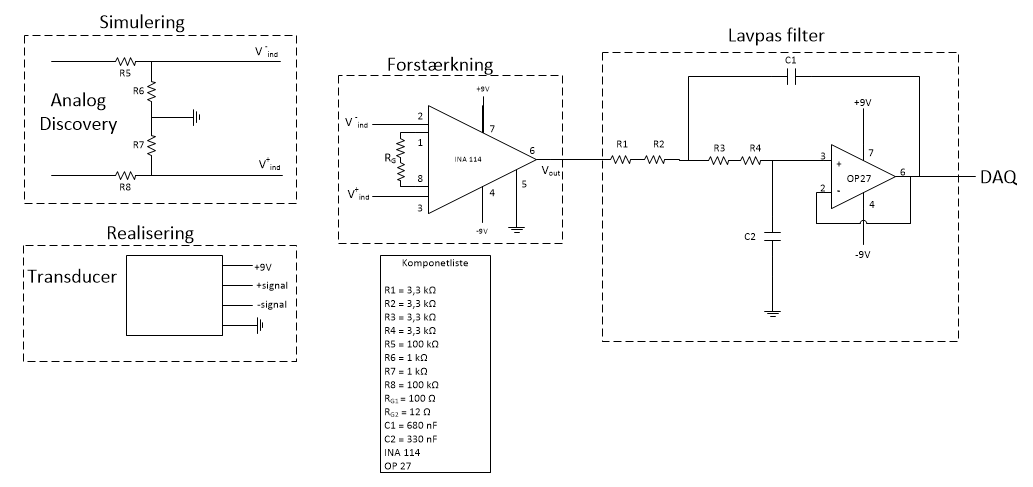
\includegraphics[width=1.0\textwidth]{Figurer/diagram_over_HW}
	\caption{Diagram over HW}
	\label{fig:HW}
\end{figure}

\subsubsection{Lavpas}
For at opnå den ønskede effekt i lavpasfilteret, blev det oplyst at $ f_c=50$ Hz, $ f_s = 1$kHz, $ R_1 = R_2 $ og $ C_2=680 nF$. Ud fra disse værdier, udregnes de resterende komponentværdier for filteret.

Overføringsfunktionen for et 2. ordens filter er: 
\begin{equation}
H(z)=\frac{\omega_n^2}{(s^2 + 2\cdot\zeta \cdot \omega_n \cdot s+\omega_n^2)}
\end{equation}

For at finde overføringsfunktionen for det gældende system, vides det at følge ligninger gælder \cite{Wikilavpas}: 
\begin{equation}
\begin{split}
\omega_n = 2\cdot \pi\ 50 = \dfrac{1}{\sqrt{R1\cdot R2\cdot C1\cdot C2}}\\
2\cdot \zeta\cdot\omega_n =\frac{1}{C2}\cdot \left( \frac{R1+R2}{R1\cdot R2}\right)
\end{split}
\end{equation}
Dette indsættes i den generelle overføringsfunktion og det simplificeres, blandt andet ved at det vides at $ R1=R2 $. 
Se Beregning af overføringsfunktion i Bilag for nærmere udregninger: 
\begin{equation}
H(z)=\dfrac{\dfrac{1}{C1 \cdot C2\cdot R^2}}{s^2+s\cdot \dfrac{2}{R\cdot C2}+ \dfrac{1}{C1\cdot C2\cdot R^2}}
\end{equation}
Når der arbejdes med et 2. ordens Butterworth filter, vides det at udsvinget$ \zeta $ skal have værdien 0.7 \cite{ASB}.
Under beregningerne, var der usikkerhed omkring, hvad værdien af $ \zeta $ skulle være. Da kredsløbet skulle realiseres og dokumenteres blev det derfor overvejet at ændre samtlige komponent værdier så de passede med en $ \zeta =1 $. Inden dette blev gjort blev det dokumenteret at det gælder at $ \zeta $ skal have en værdi på 0.7. \\
  
Den sidste overføringsfunktion sammenlignes med den generelle for 2. ordens systemer. Det gælder at $ C2 = 680\cdot 10^{-9} nF $. Det er så muligt at isolerer forskellige led. Først isoleres der for modstanden(midderste led i nævneren) og den udregnes til $ R = 6687\Omega $. \\
Nu kan det tredje led i nævner isoleres og kondensatoren $ C1 $ udregnes til $ C1 = 333 \cdot 10^{-9} nF $. \\\newline
Nærmere beregninger kan ses under Systemarkitektur i Dokumentationen. \\
Alle komponentværdierne til lavpasfilteret er fundet og det kan nu realiseres. \\ 
\newline
Under udviklingen af lavpas filteret er komponent størrelserne, blevet ændret for at kunne realisere det. De brugte komponent værdier er: $ R= 6.6 k\Omega $, $ C1= 330\cdot 10 ^{-9} nF$ og $ C2= 680\cdot 10^{-9} nF$.   
For at være sikker på at filteret har de ønskede karakteristika, laves et bodeplot for den endelig overføringsfunktion: 
\begin{equation}
H(z)=\dfrac{62500000000}{610929\cdot \left( s^2+\dfrac{250000}{561}\cdot s + \dfrac{62500000000}{610929} \right)}
\end{equation}
\begin{figure}[H]
	\centering
	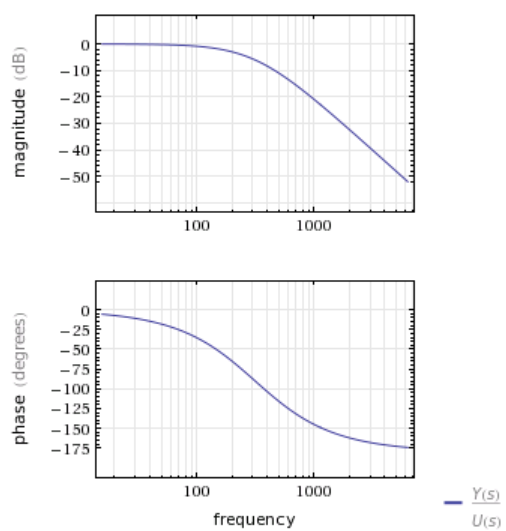
\includegraphics[width=0.5\textwidth]{Figurer/Bodeplot}
	\caption{Bodeplot}
	\label{fig:bodeplot}
\end{figure}
Ud fra den nye overføringsfunktion udregnes en nu $ \zeta $ for at kontrollere at værdien ikke har ændret sig. Denne udregnes til $ \zeta = 0.709 $. Derfor kan det konkluderes at filteret stadig har den ønskede funktionalitet. 

\subsection{Software}

\section{GUI-beskrivelse}
\subsection{Algoritmer (grænseværdier)}
\subsection{Filteret/Ufiltreret}
\subsection{Lagring af data i Database}

\section{Test}
\subsection{Hardware}
\subsubsection{Forstærkning}
For at teste forstærkningen, sendes et differentieret signal ind vha. Analog Discovery. Her observeres der hvor meget signalet bliver forstærket. 
På figur \ref{fig:forstaerkning} ses det signal, som sendes ind i forstærkningsblokken og det, der måles på udgangen af blokken. 
\begin{figure}[H]
	\centering
	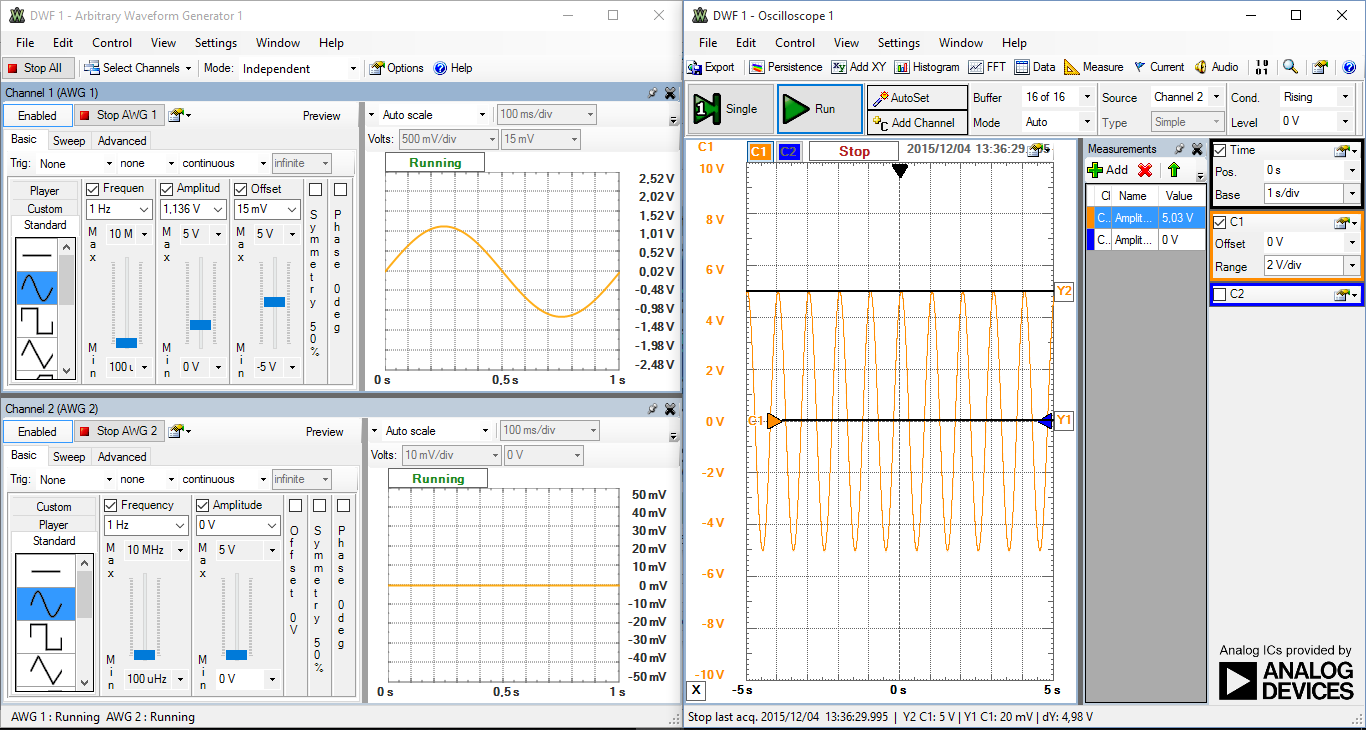
\includegraphics[width=1.0\textwidth]{Figurer/forst_blok}
	\caption{Forstærkningsblok}
	\label{fig:forstaerkning}
\end{figure}
Der sendes et differentieret signal ind i INA114. På udgangen ses det at signalet er blevet forstærket op til 5 V DC. Herved er maks. input til forstærkningsblokken blevet forstærket så det passer med maks. input til DAQ'en. Signalet bliver ikke ændret på andre måde i denne blok.

\subsubsection{Lavpas}
For at teste lavpasfilteret foretages målinger med en sinus, hvor frekvensen varierer for hver måling. Derved aflæses fasen mellem indgang- og udgangssignal, samt amplituden for hver måling. Der laves flere målinger, både før, ved og under knækfrekvensen. 
Ved knækfrekvensen skal fasedrejningen være 90\textdegree. Dette kan aflæses på figur \ref{fig:maeling50Hz}.\\
Se Modultest i Dokumentationen for mere dokumentation.  
\begin{figure}[H]
	\centering
	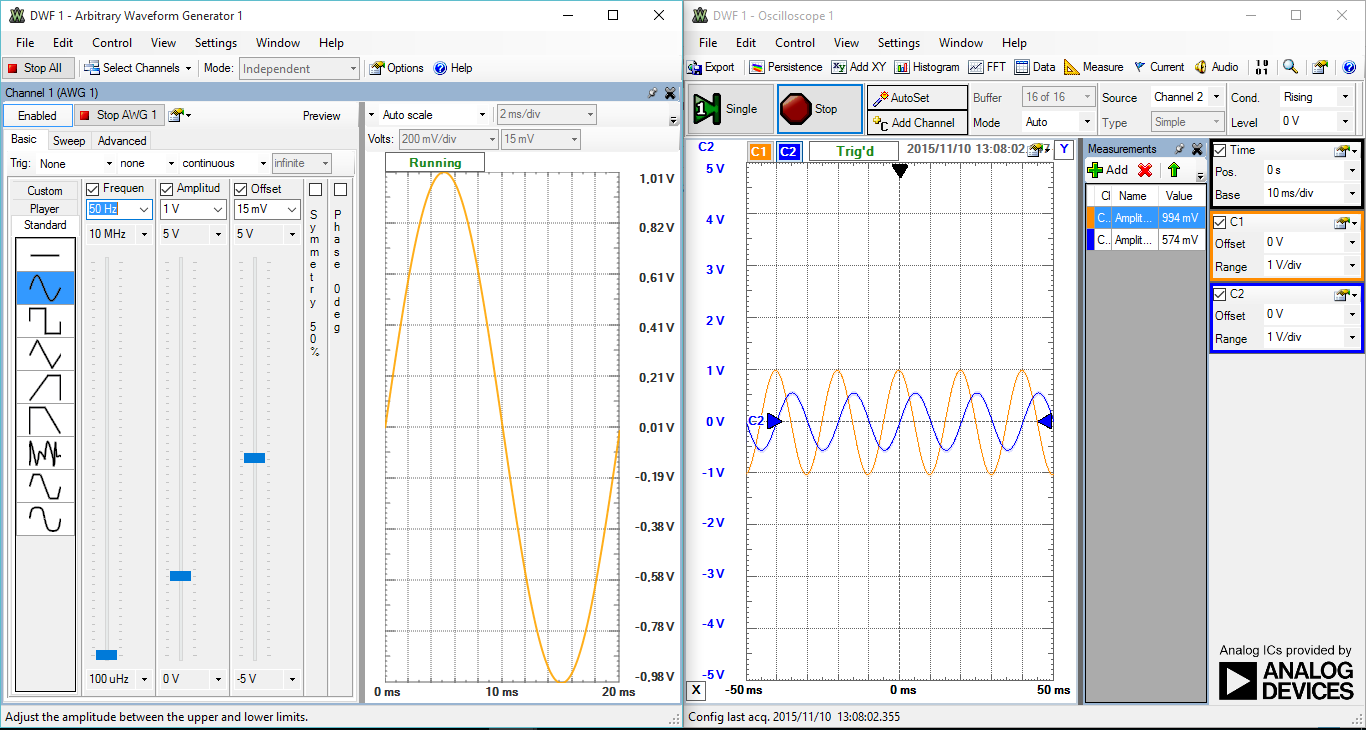
\includegraphics[width=1.0\textwidth]{Figurer/50Hz}
	\caption{Måling for 50 Hz}
	\label{fig:maeling50Hz}
\end{figure}


\subsubsection{Kalibrering med vandsøjle}
Efter forstærkning og lavpasfilteret er blevet testet hver for sig, udføres en kalibrering af systemet vha. en vandsøjle. Her bruges en udleveret vandsøjle med tre målepunkter, hvor det er angivet hvor højt trykket(målt i milimeter kviksølv, mmHg) er ved hvert af disse punkter. Derved kan det testes om hardware-delen måler den rigtige spænding i forhold til mmHg. \\
Ud fra den maksimale spænding (målt i Volt, V) og mmHg kan det udregnes, hvad hardware skal vise ved 100 mmHg, se figur \ref{fig:graf_vandtest}. 
\begin{figure}[H]
	\centering
	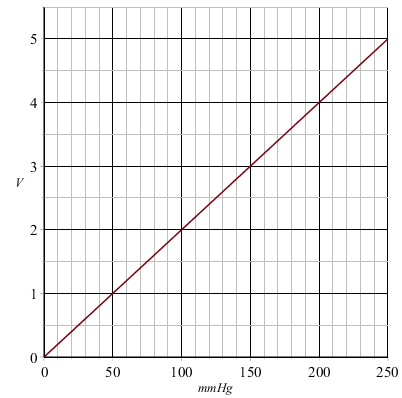
\includegraphics[width=0.3\textwidth]{Figurer/graf_vandtest}
	\caption{Graf til kalibrering, fra udregninger}
	\label{fig:graf_vandtest}
\end{figure}
Testen udføres ved at fylde vand i søjlen til et bestemt punkt. Transduceren skal være tilkoblet netop dette målepunkt, mens de andre er lukket til. Transduceren er sat til hardwaren, der hvor Analog Discovery tidligere har været sat til. Transduceren er tilkoblet 0-9V ved batterierne. På samme måde som ved simuleringen, aflæses målingen på computeren ved hjælp af programmet WaveForms. Da det vides hvilken trykændring der måles på, ved vi fra grafen til kalibreringen hvilken spænding den skal vise. Dette fortages for de tre målepunkter på vandsøjlen, hvor hver måling sammenlignes med den udregnede graf. For hver måling, skal transduceren flyttes til et af de andre målepunkter.  
\begin{figure}[H]
	\centering
	\includegraphics[width=0.3\textwidth]{Figurer/vandtest_opstilling}
	\caption{Opstilling}
	\label{fig:vandtest_opstilling}
\end{figure} 
Ud fra grafen i figur \ref{fig:graf_vandtest} vides, hvad svaret til hver måling skal være. På figur \ref{fig:vandtest_måling50} ses målingen, da transduceren var tilkoblet målepunktet for 50 mmHg. Ud fra figur \ref{fig:graf_vandtest} vides det at målingen skal vise 1 V DC.  
\begin{figure}[H]
	\centering	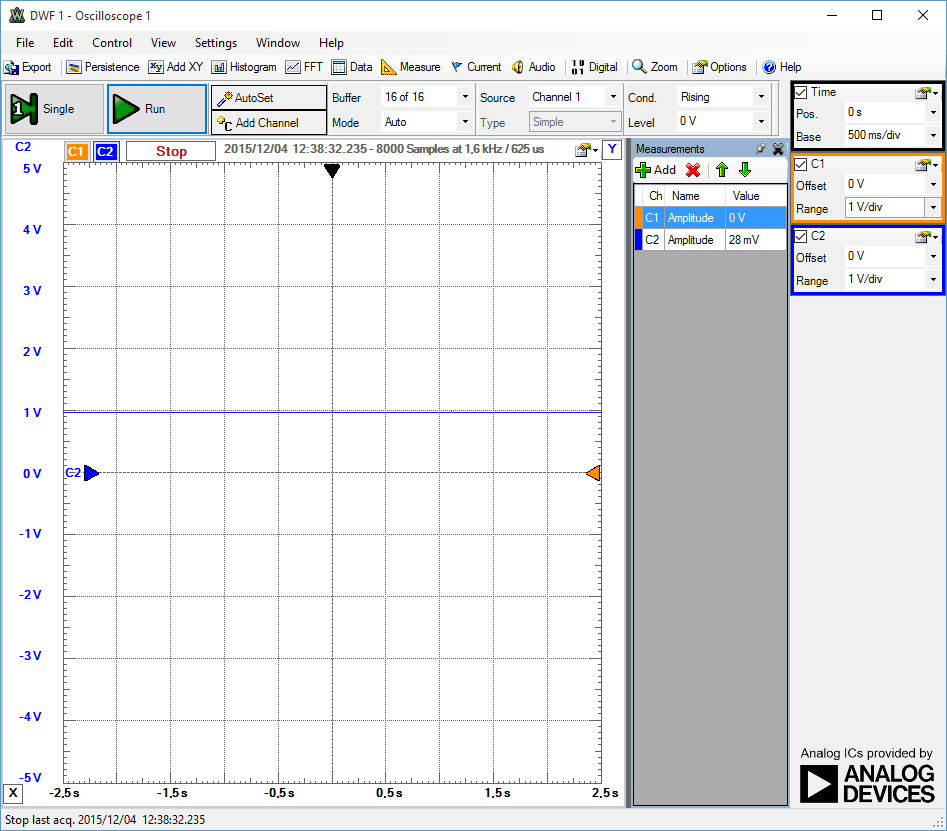
\includegraphics[width=0.6\textwidth]{Figurer/50mmhg}
	\caption{Måling ved 50 mmHg}
	\label{fig:vandtest_måling50}
\end{figure}
Ud fra figur \ref{fig:graf_vandtest} kendes udgangsspændingen også for de to andre målepunkter. Se under Modeltest i Dokumentationen for billeder af målingerne ved 10 mmHg og 100 mmHg. Målingen for 50 mmHg er her valgt ud, da denne måling ligger til baggrund for kalibreringen i softwaren. 
\subsection{Software}

\section{Resultater og diskussion}
Resultaterne for projektet er at ...

Under projektet er vores tidsplan skredet adskillige gange. Blandt andet pga. mange uforudsete problemstillinger og udefrakommende faktorer. \\Ved softwaren er det specielt teorien bag tråde og derfor forståelsen derom, som har manglet og derved skabt flere problemer. Teorien for tråde skulle være kommet i undervisningen i kurset IT3, dette har dog ikke været fyldestgørende i forhold til brugen i projektet.\\
Ved hardware har der været en manglende forståelse for de signaler som sendes ind og måles ved udgangen. Det har givet en stor usikkerhed for, hvornår de forskellige blokke har virket korrekt. Derfor er der blevet spildt tid på at tro at systemet ikke virkede, mens det i virkeligheden gjorde som det skulle.  
De udefrakommende faktorer som har spillet ind var en eksamen, som har lagt midt i det hele. Den har naturligvis være kendt hele forløbet, men det satte en stopper for projektet på ca. 1 uge.  



\section{Udviklingsværktøjer}
Gennem projektarbejdet har vi anvendt en række forskellige værktøjer til udvikling af blodtryksmåler-systemet. Disse er yderligere uddybet herunder.

\textbf{Visual Studio 2013}

Softwaredelen af projektets programmering er skrevet i sproget C-sharp. Her er Visual Studio 2013 anvendt som kompiler, da programmet gør det nemt at omskrive tekst til kode. Visual Studio 2013 indeholder også funktionen Windows Form Application, der visuelt kan fremstille de ønskede resultater i form af knapper, grafer og labels mv. i en samlet brugergrænseflade, som aktøren interagerer med. 

\textbf{Microsoft Visio 2016}

Microsoft Visio er et tegne værktøj, der i dette projekt er anvendt til at designe både SysML og UML diagrammer, som benyttes ved organisering af hardware og software design. Microsoft Visio er det oplagte valg, da diagrammer lavet i programmet får et enkelt og overskueligt udseende, og dermed fremstår det tydeligt for læseren hvad diagrammet vil vise.

\textbf{Analog Discovery og Waveform fra Digilent}

Analog Discovery og Waveform er i projektet benyttet som omformer og signal generator under testfasen. Her fungerer Analog Discovery som en Waveform generator, så et analog signal kan sendes videre ind i lavpasfiltret, forstærkeren og derefter ind i DAQ’en. I den endelig implementering erstattes Analog Discovery og Waveform med transduceren. 

\textbf{NI-DAQmx}

NI-DAQmx er et værktøj udarbejdet af National Instruments, som anvendes til at omforme det indkomne analoge signal fra transduceren (Analog Discovery) til et digital signal. Værdier fra NI-DAQmx er af en type som kan anvendes i selve softwarekoden. 

\textbf{LaTeX}

LaTeX er anvendt i projektet til design og opsætning af projektrapport og projektdokumentation. LaTeX er god til tekstformatering, hvor opsætning og strukturer defineres samlet for hele rapport, samt god til versionsstyring. Til at skrive selve koden benyttes programmet TeX-maker som kombiler. 

\section{Opnåede resultater}
\section{Perspektivering - Fremtidigt arbejde}
I fremtiden vil blodtryksmåleren kunne udvides gennem flere muligheder. Da blodtryksmåleren er lavet til forskningsbrug, er der ingen idé i at udvide mod patienter.  En forlængelse af systemet kunne derimod være en metode, som skal kunne vise gemte målinger. \newline Et log-in vindue er en anden ting, som kunne forbedre systemet, for på den måde at skabe større sikkerhed for forskeren og dataen. Et log-in vindue vil gøre at, en forsker kan være sikker på at hans målinger og forskning ikke kan tilgås af andre. Det kræver en større udvidelse, hvor der skal laves et log-in vindue og en database, hvor password og brugernavn gemmes. Der skal også laves en metode, som kan tjekke om det indtastede password og brugernavn passer over ens med det i databasen. 
\newline
Generelt skal de standarter, som findes for blodtryksmålere undersøges grundigere. Specielt brugergrænsefladen, men også resten af systemet som enheder og visning af graf, skal rettes til efter de passende standarter.
\newline 
Hvis systemet ydeligere skulle tilpasses forskning, kunne det gøres gennem en bedre navngivning af data i tabellen eller et bedre overblik over, hvordan data bliver gemt f.eks. gennem en liste for de gemte målinger. På den måde vil det blive nemmere for forskeren at finde frem til gamle målinger.   
\newline 
I forhold til hardware er målet, at det hele skal samles i en kasse. Så det på den måde ikke er muligt at ændre eller stille ved det. Derved skal filteret og forstærkningen laves på en printplade. Samtidigt skal det ved kassen være en plads til batterierne, hvor det er muligt at kunne skifte dem, når nødvendigt. Derved fås en kasse, som nemt kan flyttes rundt på og som ikke er i fare for at gå i stykker.   